
\documentclass[aspectratio=169, handout]{beamer}

%\usepackage[table]{xcolor}
\mode<presentation> {
\setbeamercovered{transparent}
  \usetheme{Boadilla}

%  \usetheme{Pittsburgh}
%\usefonttheme[2]{sans}
\renewcommand{\familydefault}{cmss}
%\usepackage{lmodern}
%\usepackage[T1]{fontenc}
%\usepackage{palatino}
%\usepackage{cmbright}
\usepackage{bm}
\usepackage{listings}
\useinnertheme{rectangles}
}
\usepackage{amsmath}
\usepackage{tcolorbox}
\setbeamercolor{normal text}{fg=black}
\setbeamercolor{structure}{fg= blue}
\definecolor{trial}{cmyk}{1,0,0, 0}
\definecolor{trial2}{cmyk}{0.00,0,1, 0}
\definecolor{darkgreen}{rgb}{0,.4, 0.1}
\definecolor{darkpurple}{rgb}{0.4, 0, 0.6}
\usepackage{array}
\beamertemplatesolidbackgroundcolor{white}  \setbeamercolor{alerted
text}{fg=darkpurple}
\setbeamertemplate{caption}[numbered]\newcounter{mylastframe}

\font\domino=domino
\def\die#1{{\domino#1}}
\usepackage{tikz}
\usetikzlibrary{arrows}
\usepackage{colortbl}

\renewcommand{\familydefault}{cmss}
%\usepackage[all]{xy}

\usepackage{tikz}
\usepackage{lipsum}
\usepackage{booktabs}
\usepackage{pifont}
\usepackage{amssymb}

\lstset{%
  language=R,
  basicstyle=\ttfamily\small,
  keywordstyle=\color{blue},
  commentstyle=\color{darkgreen},
  stringstyle=\color{red},
  showstringspaces=false,
  breaklines=true,
  frame=single,
  backgroundcolor=\color{gray!10}
}

 \newenvironment{changemargin}[3]{%
 \begin{list}{}{%
 \setlength{\topsep}{0pt}%
 \setlength{\leftmargin}{#1}%
 \setlength{\rightmargin}{#2}%
 \setlength{\topmargin}{#3}%
 \setlength{\listparindent}{\parindent}%
 \setlength{\itemindent}{\parindent}%
 \setlength{\parsep}{\parskip}%
 }%
\item[]}{\end{list}}
\usetikzlibrary{arrows}
\usetikzlibrary{arrows.meta}
\usepackage{pgfplots}
\pgfplotsset{compat=1.17}
\usecolortheme{lily}

\newtheorem{com}{Comment}
\newtheorem{lem} {Lemma}
\newtheorem{prop}{Proposition}
\newtheorem{condition}{Condition}
\newtheorem{thm}{Theorem}
\newtheorem{defn}{Definition}
\newtheorem{cor}{Corollary}
\newtheorem{obs}{Observation}
 \numberwithin{equation}{section}

\makeatletter
\def\beamerorig@set@color{%
  \pdfliteral{\current@color}%
  \aftergroup\reset@color
}
\def\beamerorig@reset@color{\pdfliteral{\current@color}}
\makeatother
\setbeamertemplate{navigation symbols}{}

\useoutertheme{miniframes}
\title[PLSC 30700]{Linear Models Lecture 10: Asymptotics}

\author{Robert Gulotty}
\institute[Chicago]{University of Chicago}
\vspace{0.3in}


\begin{document}

\begin{frame}
\maketitle
\end{frame}

%%%%%%%%%%%%%%%%%%%%%%%%%%%%%%%%%%%%%%%%%%%%%%%%%%%%%%%%%%%%
\section{Review}
\setcounter{subsection}{1}
%%%%%%%%%%%%%%%%%%%%%%%%%%%%%%%%%%%%%%%%%%%%%%%%%%%%%%%%%%%%

\begin{frame}{Big Picture}
\begin{itemize}
\item We began with a model in which $Y=\bm{x}'\bm{\beta}+e$
\item OLS finds the projection of $\bm{y}$ in the vector space spanned by $\bm{x}$:
\begin{align*}
\bm{\hat{y}}&=\bm{X\hat{\beta}}=\bm{X(X'X)^{-1}X'y}=\bm{Py}\\
\bm{\hat{e}}&=\bm{y}-\bm{\hat{y}}=\bm{y}-\bm{X\hat{\beta}}=\bm{y}-\bm{Py}=(\bm{I}-\bm{P})\bm{y}=\bm{My}
\end{align*}
\item We showed that the projection coefficient $\bm{\hat{\beta}}$ is an unbiased estimator of $\bm{\beta}$.
\item With the additional assumption of normality, we derived $t$ and $F$ distributions (Lecture 7).
\end{itemize}

\pause

\begin{tcolorbox}[colback=blue!5, colframe=blue!50]
In Lecture 9, we used asymptotic arguments \textbf{informally}: Taylor expansion of the score, LLN for the Hessian, CLT for the score. Today we develop these tools rigorously.
\end{tcolorbox}
\end{frame}

%%%%%%%%%%%%%%%%%%%%%%%%%%%%%%%%%%%%%%%%%%%%%%%%%%%%%%%%%%%%

\begin{frame}{Standards for Inference}
\begin{itemize}
\item Unbiased estimators ($E[\hat{\theta}]=\theta$) are ``correct on average'' even in small samples.
\begin{itemize}
\item Unbiasedness tells us that we are not better off with a different guess (we would lose money in expectation).
\item A biased estimator is biased even with infinite data.
\end{itemize}
\pause
\item Unbiasedness is not always what we want.
\begin{itemize}
\item Unbiasedness doesn't rule out pathological behavior: the ``first impression'' estimator is unbiased.
\item Many popular estimators are biased: Probit MLE (Lecture 9), 2SLS, ridge regression.\pause
\end{itemize}
\item A biased estimator may be a good approximation if it gets \textbf{closer to the truth with more data}.
\item What is a ``good'' approximation?
\end{itemize}
\end{frame}

%%%%%%%%%%%%%%%%%%%%%%%%%%%%%%%%%%%%%%%%%%%%%%%%%%%%%%%%%%%%

\begin{frame}{Why Consistency Matters: A Concrete Example}
U.S.\ hourly wages: $\mu = 24$, $\sigma^2 = 430$.

\begin{columns}[T]
\begin{column}{0.48\textwidth}
\textbf{``First Impression'' estimator}\\
$\hat{\mu} = X_1$ (use only the first observation)
\begin{itemize}
\item Unbiased: $\mathbb{E}[X_1] = \mu = 24$
\item $\text{Var}(\hat{\mu}) = 430$ for \emph{any} $n$
\item 95\% interval: $24 \pm 40.7$
\end{itemize}
\end{column}
\begin{column}{0.48\textwidth}
\textbf{Sample mean} $\bar{X}_n$
\begin{itemize}
\item Unbiased: $\mathbb{E}[\bar{X}_n] = \mu = 24$
\item $\text{Var}(\bar{X}_n) = 430/n \to 0$
\item 95\% interval at $n=100$: $24 \pm 4.1$
\end{itemize}
\end{column}
\end{columns}

\pause

\begin{tcolorbox}[colback=blue!5, colframe=blue!50]
Both estimators are unbiased. Only $\bar{X}_n$ is \textbf{consistent}: its distribution collapses onto $\mu$. When forced to choose, \textbf{consistency $>$ unbiasedness}.
\end{tcolorbox}
\end{frame}

%%%%%%%%%%%%%%%%%%%%%%%%%%%%%%%%%%%%%%%%%%%%%%%%%%%%%%%%%%%%

\begin{frame}

It has been customary to assume (somewhat loosely) that when a quantity is calculated from a random sample to estimate a parameter of a hypothetical frequency distribution, the accuracy of the determination will increase without limit as the number in the sample increases. A *consistent statistic* is a function of the observations actually possessing this property. \\
\hfill - Hotelling 1930


\end{frame}

%%%%%%%%%%%%%%%%%%%%%%%%%%%%%%%%%%%%%%%%%%%%%%%%%%%%%%%%%%%%

\begin{frame}{Consistency}
\begin{itemize}
\item Consistent estimators are ``more likely correct with more data''.
\item The analog to expectations in large samples is called the probability limit: $\text{plim}$.
\item Claim of Consistency: $\text{plim}\hat{\beta}=\beta$, or $\hat{\beta}_j$ is *consistent* for $\beta_j$
\end{itemize}
\end{frame}

%%%%%%%%%%%%%%%%%%%%%%%%%%%%%%%%%%%%%%%%%%%%%%%%%%%%%%%%%%%%
\section{Convergence}
%%%%%%%%%%%%%%%%%%%%%%%%%%%%%%%%%%%%%%%%%%%%%%%%%%%%%%%%%%%%

\begin{frame}{Convergence of Random Variables}

Consider the sample mean $\bar{X}_n$ as a sequence indexed by sample size $n$. Its distribution changes with $n$---how do we describe its limit?

\pause
\vspace{0.5em}

There is a hierarchy of convergence concepts for random variables:
\[
X_n \overset{\text{a.s.}}{\longrightarrow} X
\quad \Rightarrow \quad
X_n \overset{p}{\longrightarrow} X
\quad \Rightarrow \quad
X_n \overset{d}{\longrightarrow} X
\]

\pause

\begin{itemize}
  \item \textbf{Almost sure (a.s.) convergence} is the strongest form---pathwise convergence except on a probability-zero set. We won't need it operationally.

  \item \textbf{Convergence in probability} ($\overset{p}{\to}$): for all $\varepsilon > 0$, $\mathbb{P}(|X_n - X| > \varepsilon) \to 0$.
  \begin{itemize}
    \item This is the concept behind \textbf{consistency} (WLLN, plim, CMT).
  \end{itemize}

  \item \textbf{Convergence in distribution} ($\overset{d}{\to}$): $F_{X_n}(t) \to F_X(t)$ at all continuity points.
  \begin{itemize}
    \item This is the concept behind the \textbf{CLT} and asymptotic normality.
  \end{itemize}
\end{itemize}

\pause
\vspace{0.3em}
Today we develop each in turn: $\overset{p}{\to}$ (next), then $\overset{d}{\to}$ (CLT section).

\end{frame}

%%%%%%%%%%%%%%%%%%%%%%%%%%%%%%%%%%%%%%%%%%%%%%%%%%%%%%%%%%%%

\begin{frame}{Convergence in Probability}
A sequence of random variables $X_n$ converges *in probability* to $c$ if, for all $\delta>0$,
$$\lim_{n\rightarrow \infty} Pr(|X_n-c|\leq \delta)=1$$

This is written as $X_n\underset{p}{\to} c$ or $\text{plim}X_n=c$\\
We can also say
$$\lim_{n\rightarrow \infty} Pr(|X_n-c|> \delta)=0$$
That is, the random variable concentrates about a point in a certain interval.
\end{frame}

%%%%%%%%%%%%%%%%%%%%%%%%%%%%%%%%%%%%%%%%%%%%%%%%%%%%%%%%%%%%

\begin{frame}{Plim example}
\begin{itemize}
\item Define a random variable $Z_n$ that takes on values 0 and $a_n$ with probability $1-p_n$ and $p_n$ respectively, \pause
\item Intuitively $Z_n$ should converge to 0 if either $p_n\rightarrow 0$ or $a_n\rightarrow 0$.\pause
\item Consider any $\delta>0$.  If $a_n\rightarrow 0$, then for $n$ large enough, $a_n<\delta$. If so $Pr(|Z_n|\leq \delta)=1$.\pause
\item If $p_n\rightarrow 0$ then $1-p_n\rightarrow 1$.\pause
\item  $1-p_n$ of the time $Z_n=0<\delta$, so $Pr(|Z_n|\leq \delta) \geq 1-p_n$\pause
\item Therefore $Pr(|Z_n|\leq \delta)\rightarrow 1$ as $p_n\rightarrow 0$
\end{itemize}
\end{frame}

%%%%%%%%%%%%%%%%%%%%%%%%%%%%%%%%%%%%%%%%%%%%%%%%%%%%%%%%%%%%

\begin{frame}[fragile]{Consistency in Practice: OLS with Increasing $n$}

DGP: $Y_i = 2 + 3\,X_i + \varepsilon_i$, \quad $X_i \sim N(0,1)$, \quad $\varepsilon_i \sim \text{Exp}(1)-1$ (skewed, non-normal errors).

\begin{lstlisting}
set.seed(42)
par(mfrow = c(2, 2))
for (n in c(20, 50, 200, 2000)) {
  betas <- replicate(5000, {
    x <- rnorm(n); y <- 2 + 3*x + (rexp(n)-1)
    coef(lm(y ~ x))[2]
  })
  hist(betas, breaks = 40, prob = TRUE,
       main = paste("n =", n), xlim = c(2, 4),
       xlab = expression(hat(beta)[1]))
  abline(v = 3, col = "blue", lwd = 2)
}
\end{lstlisting}

\pause

Errors are \textbf{skewed and non-normal}, yet $\hat{\beta}_1$ concentrates around the true value $\beta_1 = 3$ as $n$ grows. This is consistency in action.

\end{frame}

%%%%%%%%%%%%%%%%%%%%%%%%%%%%%%%%%%%%%%%%%%%%%%%%%%%%%%%%%%%%

\begin{frame}{Why Useful : The continuous mapping theorem}
\begin{itemize}
\item Unlike expectations, plim survives continuous functions (like division!).  \pause
\end{itemize}
\begin{tcolorbox}
\textbf{The continuity theorem, the first of Slutsky's theorems, the continuous mapping theorem.}\\
Given a random variable $x_n$ that converges in probability to $x$ and a continuous function $g(x_n)$, we have that:
$$\text{plim}  g(x_n)=g(\text{plim} x_n)$$ \pause
If $\text{plim} x_n=c$ and $\text{plim} y_n=d$, then
\begin{align*}
\text{plim} (x_n y_n)&=(\text{plim} x_n)(\text{plim} y_n)=cd\\
\text{plim} (x_n/y_n)&=(\text{plim} x_n)/(\text{plim} y_n)=c/d\\
\text{plim} (x_n+y_n)&=(\text{plim} x_n)+(\text{plim} y_n)=c+d
\end{align*}
\end{tcolorbox}

\end{frame}

%%%%%%%%%%%%%%%%%%%%%%%%%%%%%%%%%%%%%%%%%%%%%%%%%%%%%%%%%%%%

\begin{frame}{CMT in Action: Why Division Works}

The $t$-statistic divides one random quantity by another. Why is this valid?

\begin{itemize}
\item WLLN: $\bar{X}_n \overset{p}{\to} \mu$ \quad and \quad $s_n^2 \overset{p}{\to} \sigma^2$
\item CMT (continuous function $g(a,b) = a/\sqrt{b}$):
\[
\frac{\bar{X}_n}{s_n} \overset{p}{\to} \frac{\mu}{\sigma}
\]
\item More generally, any smooth function of consistent estimators is itself consistent.
\end{itemize}

\pause

\begin{tcolorbox}[colback=blue!5, colframe=blue!50]
Every time you divide an estimate by its standard error, you rely on CMT. Without it, ratios of random variables have no guarantee of converging to the right thing.
\end{tcolorbox}

\end{frame}

%%%%%%%%%%%%%%%%%%%%%%%%%%%%%%%%%%%%%%%%%%%%%%%%%%%%%%%%%%%%
\section{Law of Large Numbers}
%%%%%%%%%%%%%%%%%%%%%%%%%%%%%%%%%%%%%%%%%%%%%%%%%%%%%%%%%%%%

\begin{frame}
\frametitle{Weak Law of Large Numbers}

Proof plan:
\begin{itemize}
\item[-] Markov's Inequality
\item[-] Chebyshev's Inequality
\item[-] Weak Law of Large Numbers
\end{itemize}


\end{frame}

%%%%%%%%%%%%%%%%%%%%%%%%%%%%%%%%%%%%%%%%%%%%%%%%%%%%%%%%%%%%

\begin{frame}
\frametitle{Markov's Inequality}

\begin{prop}
Suppose $X$ is a random variable that takes on non-negative values.  Then, for all $a>0$,
\begin{eqnarray}
P(X\geq a) & \leq & \frac{E[X]}{a} \nonumber
\end{eqnarray}
\end{prop}

\end{frame}

%%%%%%%%%%%%%%%%%%%%%%%%%%%%%%%%%%%%%%%%%%%%%%%%%%%%%%%%%%%%

\begin{frame}
\frametitle{Markov's Inequality}


\begin{proof}
For $a>0$,  \pause
\begin{align*}
E[X] & =  \int_{0}^{\infty} x f(x) dx \\ \pause
& =  \int_{0}^{a} x f(x) dx + \int_{a}^{\infty} x f(x) dx \\\pause
E[X] &\geq \int_{a}^{\infty} x f(x) dx  \geq \int_{a}^{\infty} a f(x)dx = a P(X \geq a ) \tag{$X\geq0$}\\ \pause
\frac{E[X]}{a} &\geq P(X \geq a )
\end{align*}


\end{proof}

\end{frame}

%%%%%%%%%%%%%%%%%%%%%%%%%%%%%%%%%%%%%%%%%%%%%%%%%%%%%%%%%%%%

\begin{frame}{Markov's Inequality: Visual Intuition}

\begin{center}
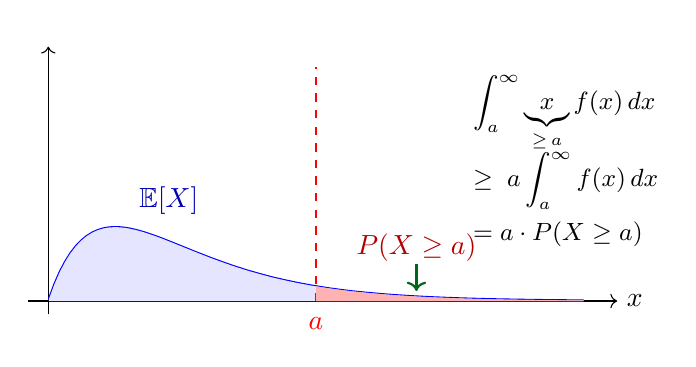
\begin{tikzpicture}[scale=0.85]
  % Axes
  \draw[->] (-0.3,0) -- (8.5,0) node[right] {$x$};
  \draw[->] (0,-0.2) -- (0,3.8) node[above] {};

  % The density f(x) — a chi-squared-like shape
  \draw[thick, blue, domain=0.01:8, samples=100]
    plot (\x, {3*\x*exp(-\x)});

  % Shade the full area under x*f(x) lightly
  \fill[blue!10, domain=0.01:8, samples=100]
    (0.01,0) -- plot (\x, {3*\x*exp(-\x)}) -- (8,0) -- cycle;

  % Mark threshold a
  \draw[dashed, red, thick] (4,0) -- (4,3.5);
  \node[below, red] at (4,-0.1) {$a$};

  % Shade tail area under f(x) for x >= a
  \fill[red!30, domain=4:8, samples=50]
    (4,0) -- plot (\x, {3*\x*exp(-\x)}) -- (8,0) -- cycle;

  % Draw the bounding rectangle: height = f evaluated at some point, width from a to ...
  % Actually, the key insight is: area under xf(x) for x>=a >= a * area under f(x) for x>=a
  % Let's show the rectangle a * P(X>=a) as a box

  % Height of the density at x=a for reference
  \pgfmathsetmacro{\fa}{3*4*exp(-4)}

  % Label the tail
  \node[red!70!black] at (5.5, 0.8) {$P(X \geq a)$};

  % Label the full area
  \node[blue!70!black] at (1.8, 1.5) {$\mathbb{E}[X]$};

  % The argument arrow
  \draw[->, thick, darkgreen] (5.5, 0.55) -- (5.5, 0.15);

  % Add annotation
  \node[right, font=\small] at (6.2, 2.8) {$\displaystyle\int_a^\infty \underbrace{x}_{\geq\, a} f(x)\,dx$};
  \node[right, font=\small] at (6.2, 1.8) {$\displaystyle\geq\; a \int_a^\infty f(x)\,dx$};
  \node[right, font=\small] at (6.2, 1.0) {$= a\cdot P(X \geq a)$};

\end{tikzpicture}
\end{center}

\pause

The full integral $\mathbb{E}[X]$ includes the \textcolor{red!70!black}{tail area}. In the tail, every $x \geq a$, so replacing $x$ with $a$ only makes the integral smaller. Hence $\mathbb{E}[X] \geq a \cdot P(X \geq a)$.

\end{frame}

%%%%%%%%%%%%%%%%%%%%%%%%%%%%%%%%%%%%%%%%%%%%%%%%%%%%%%%%%%%%

\begin{frame}
\frametitle{Chebyshev's Inequality}

\begin{prop}
If $X$ is a random variable with mean $\mu$ and variance $\sigma^2$, then, for any value $k>0$,
\begin{eqnarray}
P(|X - \mu| \geq k) & \leq & \frac{\sigma^2}{k^2} \nonumber
\end{eqnarray}

\end{prop}


\end{frame}

%%%%%%%%%%%%%%%%%%%%%%%%%%%%%%%%%%%%%%%%%%%%%%%%%%%%%%%%%%%%

\begin{frame}
\frametitle{Chebyshev's Inequality}


\begin{proof}
Define the random variable
\begin{eqnarray}
 Y & = & (X - \mu)^2 \nonumber
\end{eqnarray}

Where $\mu = E[X]$.

\pause

Then we know $Y$ is a non-negative random variable.  Set $a = k^2$ in Markov's inequality \pause
\begin{align*}
P(Y \geq k^2) &\leq \frac{E[Y]}{k^2} \\ \pause
P( (X- \mu)^2 \geq k^2) &\leq \frac{E[(X - \mu)^2]}{k^2} = \frac{\sigma^2}{k^2} \\ \pause
P( |X - \mu| \geq k) &\leq \frac{\sigma^2}{k^2}
\end{align*}
\end{proof}

\end{frame}

%%%%%%%%%%%%%%%%%%%%%%%%%%%%%%%%%%%%%%%%%%%%%%%%%%%%%%%%%%%%

\begin{frame}{Example of Markov and Chebyshev}
Suppose that we know that the number of items produced in a factory is a random variable with mean 500.
\begin{itemize}
\item How likely are we to see a production of 1000?
\item If the variance is 50, how likely is the production to be between 400 and 600?
\end{itemize}

\end{frame}

%%%%%%%%%%%%%%%%%%%%%%%%%%%%%%%%%%%%%%%%%%%%%%%%%%%%%%%%%%%%

\begin{frame}{Solution}
\begin{itemize}
\item \textbf{How likely are we to see a production of 1000?}

\textbf{Markov's Inequality:}
\[
\mathbb{P}(X \geq 1000) \leq \frac{\mathbb{E}[X]}{1000} = \frac{500}{1000} = 0.5
\]

\pause

\item \textbf{How likely is production between 400 and 600, given variance = 50?}

\textbf{Chebyshev's Inequality:}
\[
\mathbb{P}(|X - 500| \geq 100) \leq \frac{50}{100^2} = \frac{1}{200}
\]
\[
\mathbb{P}(400 \leq X \leq 600) = \mathbb{P}(|X - 500| < 100) \geq 1 - \frac{1}{200} = \frac{199}{200}
\]
\end{itemize}
\end{frame}

%%%%%%%%%%%%%%%%%%%%%%%%%%%%%%%%%%%%%%%%%%%%%%%%%%%%%%%%%%%%

\begin{frame}{Chebyshev Sample Size Calculation}
\begin{itemize}
\item U.S. hourly wages are distributed $\mu=24$ and $\sigma^2=430$,
\item How large does $n$ have to be so that $\bar{X}_n$ is within \$1 of the true mean with probability 99\%?
\begin{align*}
\mathbb{P}\left[|\bar{X}_n-\mu|\geq 1\right]&=\mathbb{P}\left[|\bar{X}_n-\mathbb{E}\left[\bar{X}_n\right]|\geq 1\right]\leq var\left[\bar{X}_n\right]=430/n\\
\frac{430}{n}&\leq .01\\
\mathbb{P}\left[|\bar{X}_n-\mu|\geq 1\right]&\leq .01 \text{ if }n=43{,}000
\end{align*}
\end{itemize}

\end{frame}

%%%%%%%%%%%%%%%%%%%%%%%%%%%%%%%%%%%%%%%%%%%%%%%%%%%%%%%%%%%%

\begin{frame}
\frametitle{Weak Law of Large Numbers}

\begin{prop}
Suppose $X_{1}, X_{2}, \hdots, X_{n}$ is iid random sample from a distribution with expectation $\mu$ and $Var(X_{i})= \sigma^2$.  Then, for all $\varepsilon >0$,
\begin{eqnarray}
P\left\{ \left| \frac{X_{1} + X_{2} + \hdots + X_{n} }{n} -\mu \right| \geq \varepsilon \right\} \rightarrow 0 \text{ as } n \rightarrow \infty \nonumber
\end{eqnarray}
or  $$\bar{X}_n\underset{p}{\to} \mathbb{E}[X]$$
\end{prop}


\end{frame}

%%%%%%%%%%%%%%%%%%%%%%%%%%%%%%%%%%%%%%%%%%%%%%%%%%%%%%%%%%%%

\begin{frame}
\frametitle{Weak Law of Large Numbers}

\begin{proof}
\begin{align*}
\frac{\text{E}[X_{1} + X_{2} + \cdots + X_{n} ]}{n}
&= \frac{\sum_{i=1}^{n} \text{E}[X_{i}] }{n} = \mu
\pause \\
\text{E}\left[ \left( \frac{\sum_{i=1}^{n} X_{i} - \mu}{n} \right)^2 \right]
&= \frac{\text{Var}(X_{1} + X_{2} + \cdots + X_{n} )}{n^2}
= \frac{ \sum_{i=1}^{n} \text{Var}(X_{i}) }{n^2}
= \frac{\sigma^2}{n}
\pause \\
\mathbb{P}\left( \left| \frac{X_{1} + X_{2} + \cdots + X_{n} }{n} - \mu \right| \geq \varepsilon \right)
&\leq \frac{\sigma^2}{n \varepsilon^2} \rightarrow 0 \quad \text{as } n \to \infty
\end{align*}
\end{proof}

\end{frame}

%%%%%%%%%%%%%%%%%%%%%%%%%%%%%%%%%%%%%%%%%%%%%%%%%%%%%%%%%%%%

\begin{frame}{WLLN interpretation}
\begin{itemize}
\item The sample mean approaches the population mean as $n\rightarrow \infty$\pause
\item General version only assumes $\mathbb{E}[X]<\infty$\pause
\item This notion that a sequence of the same sample quantity approaches a constant is called consistency.
\end{itemize}

\pause

\begin{tcolorbox}[colback=blue!5, colframe=blue!50, title=Immediate Consequence]
Any sample moment converges to its population counterpart:
\[
\frac{1}{n}\sum_{i=1}^n X_i X_i' \overset{p}{\to} \mathbb{E}[X_i X_i'], \qquad \frac{1}{n}\sum_{i=1}^n X_i Y_i \overset{p}{\to} \mathbb{E}[X_i Y_i]
\]
This is the foundation for OLS consistency (Lecture 11) and for the Probit Hessian convergence (Lecture 9).
\end{tcolorbox}

\end{frame}

%%%%%%%%%%%%%%%%%%%%%%%%%%%%%%%%%%%%%%%%%%%%%%%%%%%%%%%%%%%%

\begin{frame}{WLLN Counterexample}
\begin{itemize}
\item WLLN needs to have independent observations:\pause
\item For example, assume $X_i=Z+U_i$, like in the random effects model.\pause
\item Suppose $Z$ and $U_i$ are random and independent, $\mathbb{E}(U_i)=0$.\pause
\item $\bar{X}_n=Z+\bar{U}_n\underset{p}{\to}Z$ not a constant.
\end{itemize}
\end{frame}

%%%%%%%%%%%%%%%%%%%%%%%%%%%%%%%%%%%%%%%%%%%%%%%%%%%%%%%%%%%%
\section{Asymptotic Order Notation}
\setcounter{subsection}{1}
%%%%%%%%%%%%%%%%%%%%%%%%%%%%%%%%%%%%%%%%%%%%%%%%%%%%%%%%%%%%

\begin{frame}{Big $O$ and Little $o$: The Idea}

When we take limits, we often need to say ``this term is negligible compared to that one.'' Asymptotic notation gives us a precise language for this.

\pause

\begin{itemize}
\item Consider $f(n) = 3n^2 + 5n + 7$ as $n \to \infty$. \pause
\item For large $n$, the $3n^2$ term dominates: at $n = 100$, we have $30{,}000 + 500 + 7$. \pause
\item We want to say: ``$f(n)$ \emph{grows like} $n^2$'' and ``the $5n + 7$ part is \emph{negligible} relative to $n^2$.''
\end{itemize}

\pause

Two notions of ``negligible'':
\begin{itemize}
  \item \textbf{Little $o$} = ``\emph{vanishes} relative to'': \quad $a_n$ shrinks \emph{faster} than $b_n$
  \item \textbf{Big $O$} = ``\emph{bounded} relative to'': \quad $a_n$ grows \emph{no faster} than $b_n$
\end{itemize}

\pause

\begin{tcolorbox}[colback=blue!5, colframe=blue!50]
Analogy: if $b_n$ is a speed limit, then $a_n = o(b_n)$ means $a_n$ is slowing to a stop, while $a_n = O(b_n)$ means $a_n$ is obeying the speed limit (but may still be driving).
\end{tcolorbox}

\end{frame}

%%%%%%%%%%%%%%%%%%%%%%%%%%%%%%%%%%%%%%%%%%%%%%%%%%%%%%%%%%%%

\begin{frame}{Formal Definitions: $O$ and $o$}

\begin{defn}
Let $\{a_n\}$ and $\{b_n\}$ be sequences with $b_n > 0$.
\begin{itemize}
  \item \textbf{Little $o$:} \quad $a_n = o(b_n)$ \quad means \quad $\displaystyle\frac{a_n}{b_n} \to 0$ \quad as $n \to \infty$.

  \medskip

  \item \textbf{Big $O$:} \quad $a_n = O(b_n)$ \quad means \quad $\displaystyle\left|\frac{a_n}{b_n}\right| \leq C$ \quad for some constant $C$ and all $n$ large enough.
\end{itemize}
\end{defn}

\pause

\textbf{In words:}
\begin{itemize}
  \item $a_n = o(b_n)$: ``$a_n$ vanishes compared to $b_n$'' \quad (the ratio goes to zero)
  \item $a_n = O(b_n)$: ``$a_n$ is at most on the order of $b_n$'' \quad (the ratio stays bounded)
\end{itemize}

\pause

Note: little $o$ is a \emph{stronger} statement than big $O$. If $a_n = o(b_n)$ then $a_n = O(b_n)$, but not vice versa.

\end{frame}

%%%%%%%%%%%%%%%%%%%%%%%%%%%%%%%%%%%%%%%%%%%%%%%%%%%%%%%%%%%%

\begin{frame}{Examples: $O$ and $o$ with Sequences}

\renewcommand{\arraystretch}{1.6}
\begin{tabular}{lll}
\toprule
\textbf{Statement} & \textbf{Check} & \textbf{Why} \\
\midrule
$5n = o(n^2)$ & $5n/n^2 = 5/n \to 0$ \checkmark & $n$ grows slower than $n^2$ \\
$5n = O(n^2)$ & $5n/n^2 = 5/n \leq 5$ \checkmark & also bounded (weaker) \\
$3n^2 = O(n^2)$ & $3n^2/n^2 = 3$ \checkmark & bounded but doesn't vanish \\
$3n^2 = o(n^2)$? & $3n^2/n^2 = 3 \not\to 0$ \ding{55} & same order, not negligible \\
$1/n = o(1)$ & $\frac{1/n}{1} \to 0$ \checkmark & $1/n$ vanishes \\
$1/n^2 = o(1/n)$ & $\frac{1/n^2}{1/n} = 1/n \to 0$ \checkmark & $1/n^2$ vanishes faster \\
\bottomrule
\end{tabular}
\renewcommand{\arraystretch}{1.0}

\pause

\bigskip

\textbf{The punchline for this course:} When we write $f(x) = g(x) + O(x^3)$, we mean the leftover terms are \emph{at most} on the order of $x^3$. When $x$ is small (like $t/\sqrt{n}$), these terms are negligible.

\end{frame}

%%%%%%%%%%%%%%%%%%%%%%%%%%%%%%%%%%%%%%%%%%%%%%%%%%%%%%%%%%%%

\begin{frame}{Application: Taylor Remainder in $O$ Notation}

Consider the Taylor expansion of $\ln(1+x)$ around $x = 0$:
$$\ln(1 + x) = x - \frac{x^2}{2} + \frac{x^3}{3} - \cdots$$

\pause

We can truncate and describe what we dropped:
\begin{align*}
\ln(1+x) &= x + O(x^2) \tag{first-order: remainder $\leq C x^2$} \\
\ln(1+x) &= x - \frac{x^2}{2} + O(x^3) \tag{second-order: remainder $\leq C x^3$}
\end{align*}

\pause

\textbf{Why this is useful:} If $x = t/\sqrt{n}$, then:
\begin{itemize}
  \item $O(x^2) = O(1/n)$ --- vanishes as $n$ grows
  \item $O(x^3) = O(n^{-3/2})$ --- vanishes even faster
\end{itemize}

\pause

This is exactly how we will control the error in the CLT proof: the Taylor remainder in the MGF expansion becomes negligible as $n \to \infty$.

\end{frame}

%%%%%%%%%%%%%%%%%%%%%%%%%%%%%%%%%%%%%%%%%%%%%%%%%%%%%%%%%%%%

\begin{frame}{Big $O_p$ and Little $o_p$: The Stochastic Versions}

For \emph{random} variables, we add a subscript $p$ (``in probability''):

\begin{defn}
\begin{itemize}
  \item $X_n = o_p(a_n)$: \quad $X_n/a_n \overset{p}{\to} 0$ \quad (``vanishes in probability'')
  \item $X_n = O_p(a_n)$: \quad $X_n/a_n$ stays \emph{bounded in probability}
\end{itemize}
\end{defn}

\pause

\textbf{Translations to what we just proved:}
\begin{itemize}
  \item $X_n \overset{p}{\to} c$ is the same as writing $X_n - c = o_p(1)$
  \item WLLN says $\bar{X}_n - \mu = o_p(1)$, and more precisely $\bar{X}_n - \mu = O_p(n^{-1/2})$
  \item CLT (coming next) says $\sqrt{n}(\bar{X}_n - \mu) = O_p(1)$
\end{itemize}

\pause

\begin{tcolorbox}[colback=blue!5, colframe=blue!50]
When you see $o_p(1)$ in a proof, read it as ``a term that vanishes in probability --- we can ignore it.''
\end{tcolorbox}

\end{frame}

%%%%%%%%%%%%%%%%%%%%%%%%%%%%%%%%%%%%%%%%%%%%%%%%%%%%%%%%%%%%
\section{Mathematical Tools for the CLT}
\setcounter{subsection}{1}
%%%%%%%%%%%%%%%%%%%%%%%%%%%%%%%%%%%%%%%%%%%%%%%%%%%%%%%%%%%%

\begin{frame}{What is a Taylor Expansion?}

\textbf{Problem:} We know everything about a function $f$ at a point $a$ (its value, slope, curvature, \ldots), and we want to approximate $f$ at a \emph{nearby} point $b$.

\pause

\textbf{Idea:} Build the approximation one piece at a time:
\begin{enumerate}
  \item \textbf{Zeroth order:} Start with $f(b) \approx f(a)$ \quad (constant --- ignore everything)
  \item \textbf{First order:} Add the slope: $f(b) \approx f(a) + f'(a)(b-a)$ \quad (tangent line)
  \item \textbf{Second order:} Add the curvature: $f(b) \approx f(a) + f'(a)(b-a) + \frac{f''(a)}{2}(b-a)^2$
  \item Keep going: each term uses one more derivative and improves the fit near $a$.
\end{enumerate}

\pause

\begin{tcolorbox}[colback=blue!5, colframe=blue!50]
\textbf{Key insight:} The closer $b$ is to $a$, the better the approximation. If $b - a$ is small, then $(b-a)^2$ is \emph{very} small, $(b-a)^3$ is \emph{tiny}, etc. --- so the first few terms do most of the work.
\end{tcolorbox}

\end{frame}

%%%%%%%%%%%%%%%%%%%%%%%%%%%%%%%%%%%%%%%%%%%%%%%%%%%%%%%%%%%%

\begin{frame}{Taylor Approximation: First Order}

\begin{itemize}
\item We know $f(a)$ and $f'(a)$. We want to approximate $f(b)$ for $b$ near $a$. \pause
\item \textbf{First-order Taylor expansion:}
$$f(b) = f(a) + f'(a)(b - a) + R_1(b)$$
where the remainder $R_1(b) = \frac{f''(c)}{2}(b-a)^2$ for some $c$ between $a$ and $b$.

\pause

\item In asymptotic-order notation:
$$f(b) = f(a) + f'(a)(b - a) + O\!\left((b-a)^2\right)$$
\end{itemize}

\begin{center}
\includegraphics[width=3.5in]{approx.png}
\end{center}

\end{frame}

%%%%%%%%%%%%%%%%%%%%%%%%%%%%%%%%%%%%%%%%%%%%%%%%%%%%%%%%%%%%

\begin{frame}{Taylor Approximation: Higher Orders}

The $k$-th order Taylor expansion of $f$ around $a$:
$$f(b) = \sum_{j=0}^{k} \frac{f^{(j)}(a)}{j!}(b-a)^j + O\!\left((b-a)^{k+1}\right)$$

\pause

\textbf{Second-order expansion} (used constantly in asymptotic theory):
$$f(b) = f(a) + f'(a)(b-a) + \frac{f''(a)}{2}(b-a)^2 + O\!\left((b-a)^3\right)$$

\pause

\textbf{Why this matters:}
\begin{itemize}
  \item The \textbf{Delta Method} uses the first-order expansion to linearize functions of estimators.
  \item The \textbf{CLT proof} uses the second-order expansion of the moment generating function.
  \item The $O(\cdot)$ notation tells us exactly which terms we can drop as $n \to \infty$.
\end{itemize}

\end{frame}

%%%%%%%%%%%%%%%%%%%%%%%%%%%%%%%%%%%%%%%%%%%%%%%%%%%%%%%%%%%%

\begin{frame}{The Exponential Function as a Series}

The most important function in mathematics is $\exp(x)$, \emph{defined} by:
$$\exp(x) = \sum_{k=0}^{\infty} \frac{x^k}{k!} = 1 + x + \frac{x^2}{2!} + \frac{x^3}{3!} + \cdots$$

\pause

\textbf{Key properties (all follow from the series):}
\begin{enumerate}
\item $\exp(a)\exp(b) = \exp(a+b)$, so we write $e^x \equiv \exp(x)$ where $e = \exp(1) = 2.718\ldots$
\item $\frac{d}{dx}e^x = e^x$: differentiate term-by-term and re-index. \pause
\item The series \emph{is} the Taylor expansion of $e^x$ around 0 (since every derivative is $e^x$ and $e^0=1$).
\end{enumerate}

\pause

\begin{tcolorbox}[colback=blue!5, colframe=blue!50]
\textbf{Why this matters now:} We will expand $\mathbb{E}[e^{tX}]$ using this series to extract moments, and then use the Taylor remainder to control the error in the CLT proof.
\end{tcolorbox}

\end{frame}

%%%%%%%%%%%%%%%%%%%%%%%%%%%%%%%%%%%%%%%%%%%%%%%%%%%%%%%%%%%%

\begin{frame}{The Compound Interest Limit}

\begin{prop}
$\displaystyle\lim_{n \to \infty}\left(1 + \frac{x}{n}\right)^n = e^x$
\end{prop}

\pause

\textbf{Proof:} Take logs, apply the Taylor expansion $\ln(1+u) = u - \frac{u^2}{2} + O(u^3)$:
\begin{align*}
n \ln\!\left(1 + \frac{x}{n}\right) &= n\!\left(\frac{x}{n} - \frac{x^2}{2n^2} + O(n^{-3})\right) = x - \frac{x^2}{2n} + O(n^{-2}) \to x
\end{align*}
So $\left(1 + \frac{x}{n}\right)^n = e^{n\ln(1+x/n)} \to e^x$.

\pause

\begin{tcolorbox}[colback=blue!5, colframe=blue!50]
This converts a product of $n$ nearly-identical terms into an exponential --- the crucial step in the CLT proof: $(1 + t^2/(2n) + \text{small})^n \to e^{t^2/2}$.
\end{tcolorbox}

\end{frame}

%%%%%%%%%%%%%%%%%%%%%%%%%%%%%%%%%%%%%%%%%%%%%%%%%%%%%%%%%%%%

\begin{frame}{Moment Generating Functions}

\begin{defn}
The \textbf{moment generating function} (MGF) of a random variable $X$ is:
$$M_X(t) = \mathbb{E}[e^{tX}]$$
defined for all $t$ in a neighborhood of $0$.
\end{defn}

\pause

\textbf{Why ``moment generating''?} Expand $e^{tX}$ using the series definition:
\begin{align*}
M_X(t) &= \mathbb{E}\!\left[\sum_{k=0}^{\infty} \frac{(tX)^k}{k!}\right] = \sum_{k=0}^{\infty} \frac{t^k}{k!}\,\mathbb{E}[X^k]\\
&= 1 + t\,\mathbb{E}[X] + \frac{t^2}{2}\,\mathbb{E}[X^2] + \cdots
\end{align*}

\pause

So $M_X^{(k)}(0) = \mathbb{E}[X^k]$: the $k$-th derivative at zero gives the $k$-th moment.

\end{frame}

%%%%%%%%%%%%%%%%%%%%%%%%%%%%%%%%%%%%%%%%%%%%%%%%%%%%%%%%%%%%

\begin{frame}{MGFs: Key Properties}

\textbf{Why MGFs are useful for proving limit theorems:}

\begin{enumerate}
  \item \textbf{Uniqueness:} If $M_X(t) = M_Y(t)$ in a neighborhood of $0$, then $X$ and $Y$ have the same distribution. \pause
  \item \textbf{Independence:} If $X$ and $Y$ are independent, $M_{X+Y}(t) = M_X(t) \cdot M_Y(t)$.
  \begin{itemize}
    \item For $n$ iid copies: $M_{X_1 + \cdots + X_n}(t) = [M_{X_1}(t)]^n$
  \end{itemize} \pause
  \item \textbf{Continuity theorem:} If $M_{X_n}(t) \to M_X(t)$ for all $t$ near $0$, then $X_n \overset{d}{\to} X$.
\end{enumerate}

\pause

\begin{tcolorbox}[colback=blue!5, colframe=blue!50]
\textbf{Standard normal MGF:} If $Z \sim N(0,1)$, then $M_Z(t) = e^{t^2/2}$.\\[4pt]
\textbf{Proof strategy for CLT:} Show that the MGF of the standardized sample mean converges to $e^{t^2/2}$.
\end{tcolorbox}

\end{frame}

%%%%%%%%%%%%%%%%%%%%%%%%%%%%%%%%%%%%%%%%%%%%%%%%%%%%%%%%%%%%
\section{Central Limit Theory}
%%%%%%%%%%%%%%%%%%%%%%%%%%%%%%%%%%%%%%%%%%%%%%%%%%%%%%%%%%%%

\begin{frame}{Convergence in Distribution}
\begin{itemize}
\item We want the sampling distribution of the sample mean $\bar{X}_n$.
\item The sampling distribution is a function of the distribution of observations $F$ and the sample size $n$.
\item We will get an \emph{asymptotic approximation} by standardizing $\bar{X}_n$ and taking the limit as $n\to \infty$
\end{itemize}
\end{frame}

%%%%%%%%%%%%%%%%%%%%%%%%%%%%%%%%%%%%%%%%%%%%%%%%%%%%%%%%%%%%

\begin{frame}{Definition: Convergence in Distribution}
\begin{itemize}
  \item Let \( X_n \) be a sequence of random variables, and \( X \) a target random variable.
  \item We say that \( X_n \) \textbf{converges in distribution} to \( X \) if:
  \[
  \lim_{n \to \infty} \mathbb{P}(X_n \leq t) = \mathbb{P}(X \leq t) \quad \text{for all } t \text{ where } F_X(t) \text{ is continuous}
  \]

  \item \textbf{Implications}
  \begin{itemize}
    \item The cumulative distribution functions converge: \( F_{X_n}(t) \to F_X(t) \)
    \item If the target distribution is a constant, then this is just convergence in probability
  \end{itemize}
  \item \textbf{Notation:} \quad \( X_n \underset{d}{\to} X \)
\end{itemize}
\end{frame}

%%%%%%%%%%%%%%%%%%%%%%%%%%%%%%%%%%%%%%%%%%%%%%%%%%%%%%%%%%%%

\begin{frame}{Standardizing the Sample Mean}
\begin{itemize}
\item The WLLN tells us that $\bar{X}_n\underset{p}{\to} \mu$, so $\bar{X}_n\underset{d}{\to} \mu$.
\item But the distribution of $\mu$ is degenerate,  not useful.
\item So rescale by the variance: $var[\bar{X}_n-\mu]=\frac{\sigma^2}{n}$, so $var[\sqrt{n}(\bar{X}_n-\mu)]=\sigma^2$
$$Z_n=\sqrt{n}(\bar{X}_n-\mu)$$
\item As $n\to \infty$, $\mathbb{E}[Z_n]\rightarrow0$, $\mathbb{E}[Z_n^2]\rightarrow\sigma^2$, $\mathbb{E}[Z_n^3]\rightarrow0$, $\mathbb{E}[Z_n^4]\rightarrow 3\sigma^4$
\item The Central Limit Theorem states that $Z_n\underset{d}{\to}Z$ where $Z\sim N(0, \sigma^2)$.
\item This means that $\bar{X}_n\underset{a}{\sim}N(\mu,\ \frac{\sigma^2}{n})$.
\end{itemize}
\end{frame}

%%%%%%%%%%%%%%%%%%%%%%%%%%%%%%%%%%%%%%%%%%%%%%%%%%%%%%%%%%%%

\begin{frame}{The Central Limit Theorem}

\begin{thm}[Lindeberg--L\'evy CLT]
Let $X_1, X_2, \ldots$ be iid with $\mathbb{E}[X_i] = \mu$ and $\operatorname{Var}(X_i) = \sigma^2 < \infty$. Then:
\[
\sqrt{n}(\bar{X}_n - \mu) \overset{d}{\to} N(0, \sigma^2)
\]
Equivalently: $\frac{\bar{X}_n - \mu}{\sigma/\sqrt{n}} \overset{d}{\to} N(0, 1)$.
\end{thm}

\pause

\textbf{Key conditions:}
\begin{itemize}
    \item \textbf{iid} --- can be relaxed (Lindeberg--Feller allows heterogeneity)
    \item \textbf{Finite variance} --- essential; without it, convergence may fail or be to a non-normal limit
\end{itemize}

\pause

\textbf{Remarkable fact:} The limit distribution is $N(0,\sigma^2)$ \textbf{regardless} of the distribution of $X_i$. Whether the data are Bernoulli, exponential, or uniform, the sample mean is approximately normal for large $n$.

\end{frame}

%%%%%%%%%%%%%%%%%%%%%%%%%%%%%%%%%%%%%%%%%%%%%%%%%%%%%%%%%%%%

\begin{frame}{Proof of the CLT: Setup}

\textbf{Goal:} Show $Z_n = \frac{\bar{X}_n - \mu}{\sigma/\sqrt{n}} \overset{d}{\to} N(0,1)$.

\pause

\textbf{Strategy:} Show that $M_{Z_n}(t) \to e^{t^2/2}$, the MGF of $N(0,1)$.

\pause

\textbf{Step 1.} Let $W_i = \frac{X_i - \mu}{\sigma}$, so $\mathbb{E}[W_i] = 0$ and $\mathbb{E}[W_i^2] = 1$. Then:
$$Z_n = \frac{1}{\sqrt{n}} \sum_{i=1}^n W_i$$

\pause

\textbf{Step 2.} By independence:
$$M_{Z_n}(t) = \left[M_{W}\!\left(\frac{t}{\sqrt{n}}\right)\right]^n$$

\pause

We need to evaluate $M_W(t/\sqrt{n})$ for large $n$, i.e., for small argument. This is where Taylor expansion enters.

\end{frame}

%%%%%%%%%%%%%%%%%%%%%%%%%%%%%%%%%%%%%%%%%%%%%%%%%%%%%%%%%%%%

\begin{frame}{Proof of the CLT: Taylor Expansion of the MGF}

\textbf{Step 3.} Taylor-expand $M_W(s)$ around $s = 0$:
$$M_W(s) = M_W(0) + M_W'(0)\,s + \frac{M_W''(0)}{2}\,s^2 + O(s^3)$$

\pause

Recall: $M_W^{(k)}(0) = \mathbb{E}[W^k]$. Since $\mathbb{E}[W] = 0$ and $\mathbb{E}[W^2] = 1$:
$$M_W(s) = 1 + 0 \cdot s + \frac{1}{2}\,s^2 + O(s^3) = 1 + \frac{s^2}{2} + O(s^3)$$

\pause

\textbf{Step 4.} Substitute $s = t/\sqrt{n}$:
$$M_W\!\left(\frac{t}{\sqrt{n}}\right) = 1 + \frac{t^2}{2n} + O(n^{-3/2})$$

\pause

\textbf{Step 5.} Raise to the $n$-th power:
$$M_{Z_n}(t) = \left[1 + \frac{t^2}{2n} + O(n^{-3/2})\right]^n$$

\end{frame}

%%%%%%%%%%%%%%%%%%%%%%%%%%%%%%%%%%%%%%%%%%%%%%%%%%%%%%%%%%%%

\begin{frame}{Proof of the CLT: The Exponential Limit}

\textbf{Step 6.} Apply the limit $(1 + x/n)^n \to e^x$:

$$M_{Z_n}(t) = \left[1 + \frac{t^2/2}{n} + O(n^{-3/2})\right]^n \longrightarrow e^{t^2/2}$$

\pause

\begin{itemize}
  \item The $O(n^{-3/2})$ remainder vanishes faster than $1/n$, so it does not affect the limit.
  \item The limit $e^{t^2/2}$ is precisely the MGF of $N(0,1)$.
\end{itemize}

\pause

\textbf{Step 7.} By the continuity theorem for MGFs:
$$Z_n = \frac{\sqrt{n}(\bar{X}_n - \mu)}{\sigma} \overset{d}{\to} N(0,1) \qquad \blacksquare$$

\pause

\begin{tcolorbox}[colback=blue!5, colframe=blue!50]
\textbf{What made this work:} Taylor expansion gave us $1 + t^2/(2n) + \text{small}$; the exponential limit turned a product of $n$ terms into $e^{t^2/2}$; the MGF continuity theorem converted convergence of transforms into convergence in distribution.
\end{tcolorbox}

\end{frame}

%%%%%%%%%%%%%%%%%%%%%%%%%%%%%%%%%%%%%%%%%%%%%%%%%%%%%%%%%%%%

\begin{frame}{CLT Sample Size Calculation}
\begin{itemize}
\item U.S. wages are distributed $\mu=24$ and $\sigma^2=430$, so $\bar{X}_n\underset{a}{\to} N(24, .43)$ for n=1000.
\item How large does $n$ have to be so that $\bar{X}_n$ is within \$1 of the true mean with 99\% probability?
\begin{align*}
\mathbb{P}\left[ |\bar{X}_n-\mu|\geq 1\right] &\underset{a}{\sim} \mathbb{P}\left[ |N(0,1)|\geq 1/\sqrt{var(\bar{X}_n)}\right]=\mathbb{P}\left[ |N(0,1)|\geq 1/\sqrt{\frac{430}{n}}\right]=.01\\
\mathbb{P}(|Z| \geq z)&=.01\rightarrow qnorm(.005)= -2.576\\
\frac{1}{\sqrt{430/n}}&=2.576\\
n&=\frac{430}{(1/2.576)^2}\\
n&\geq 2{,}862
\end{align*}
\end{itemize}

\pause

Compare with Chebyshev: $n = 43{,}000$. The CLT is far more efficient because it uses the shape of the distribution, not just the variance.

\end{frame}

%%%%%%%%%%%%%%%%%%%%%%%%%%%%%%%%%%%%%%%%%%%%%%%%%%%%%%%%%%%%

\begin{frame}[fragile]{CLT in Action: R Simulation}

\begin{lstlisting}
# CLT: sample means of Exponential(1) converge to Normal
set.seed(42)
par(mfrow = c(2, 2))
for (n in c(5, 30, 100, 1000)) {
  xbar <- replicate(10000, mean(rexp(n, rate = 1)))
  hist(xbar, breaks = 40, prob = TRUE,
       main = paste("n =", n),
       xlab = expression(bar(X)[n]))
  curve(dnorm(x, 1, 1/sqrt(n)), add = TRUE,
        col = "red", lwd = 2)
}
\end{lstlisting}

\pause

The red curve is the normal approximation $N(\mu, \sigma^2/n)$. Even for \textbf{skewed} distributions (Exponential), the normal approximation is excellent by $n = 30$.

\end{frame}

%%%%%%%%%%%%%%%%%%%%%%%%%%%%%%%%%%%%%%%%%%%%%%%%%%%%%%%%%%%%

\begin{frame}{When Do Asymptotics Kick In?}

\begin{center}
\renewcommand{\arraystretch}{1.4}
\begin{tabular}{>{\raggedright}p{3.5cm} l l}
\toprule
\textbf{Data shape} & \textbf{Rule of thumb} & \textbf{Example} \\
\midrule
Symmetric, light tails & $n \geq 30$ & Heights, test scores \\
Moderate skew & $n \geq 100$ & Wages, income \\
Heavy tails / outliers & $n \geq 500{+}$ & Financial returns, conflict \\
Rare binary outcome & Events $\geq 10$/covariate & Coups, wars \\
\bottomrule
\end{tabular}
\renewcommand{\arraystretch}{1.0}
\end{center}

\pause

\begin{tcolorbox}[colback=blue!5, colframe=blue!50]
There is no universal rule. The CLT convergence rate depends on the \textbf{shape} of the underlying distribution. When in doubt, \textbf{simulate}.
\end{tcolorbox}

\end{frame}

%%%%%%%%%%%%%%%%%%%%%%%%%%%%%%%%%%%%%%%%%%%%%%%%%%%%%%%%%%%%

\begin{frame}{Multivariate CLT}

The CLT generalizes to vectors. If $\bm{W}_1, \ldots, \bm{W}_n$ are iid $k$-vectors with $\mathbb{E}[\bm{W}_i] = \bm{\mu}$ and $\operatorname{Var}(\bm{W}_i) = \bm{\Sigma}$, then:
\[
\sqrt{n}(\bar{\bm{W}}_n - \bm{\mu}) \overset{d}{\to} N(\bm{0}, \bm{\Sigma})
\]

\pause

\textbf{Applications:}
\begin{itemize}
    \item \textbf{OLS} (Lecture 11): $\frac{1}{\sqrt{n}} \sum_{i=1}^n X_i e_i \overset{d}{\to} N(\bm{0},\, \sigma^2 Q_{XX})$

    \item \textbf{Probit MLE} (Lecture 9): $\frac{1}{\sqrt{n}} S_n(\beta_0) \overset{d}{\to} N(\bm{0},\, \mathcal{I}(\beta_0))$

    \item \textbf{GMM} (coming later): $\frac{1}{\sqrt{n}} \sum_{i=1}^n g(W_i, \theta_0) \overset{d}{\to} N(\bm{0},\, \Omega)$
\end{itemize}

\pause

In each case, a sum of mean-zero random vectors converges to a multivariate normal. The covariance matrix differs, but the \textbf{structure} is identical.

\end{frame}

%%%%%%%%%%%%%%%%%%%%%%%%%%%%%%%%%%%%%%%%%%%%%%%%%%%%%%%%%%%%
\section{Summary and Looking Ahead}
%%%%%%%%%%%%%%%%%%%%%%%%%%%%%%%%%%%%%%%%%%%%%%%%%%%%%%%%%%%%

\begin{frame}{What We Developed Today}

\begin{center}
\renewcommand{\arraystretch}{1.3}
\begin{tabular}{lll}
\toprule
\textbf{Tool} & \textbf{Statement} & \textbf{Application} \\
\midrule
WLLN & $\bar{X}_n \overset{p}{\to} \mu$ & Consistency \\
CMT & $\text{plim}\, g(X_n) = g(\text{plim}\, X_n)$ & Functions of estimators \\
$O_p$, $o_p$ & Rate of convergence & Tracking remainders \\
CLT & $\sqrt{n}(\bar{X}_n - \mu) \overset{d}{\to} N(0,\sigma^2)$ & Asymptotic normality \\
\bottomrule
\end{tabular}
\renewcommand{\arraystretch}{1.0}
\end{center}

\pause

\textbf{The CLT proof brought together:}
\begin{enumerate}
\item Taylor expansion of the MGF (second-order approximation)
\item $O(\cdot)$ notation to track the remainder
\item The exponential limit $(1 + x/n)^n \to e^x$
\item MGF continuity theorem to conclude convergence in distribution
\end{enumerate}

\end{frame}

%%%%%%%%%%%%%%%%%%%%%%%%%%%%%%%%%%%%%%%%%%%%%%%%%%%%%%%%%%%%

\begin{frame}{Looking Ahead}

\textbf{Lecture 11} introduces the \textbf{Delta Method} and applies all of today's tools to OLS:
\begin{itemize}
    \item \textbf{Delta Method}: Taylor expansion + CLT $\Rightarrow$ distribution of $h(\hat\beta)$
    \item \textbf{Consistency}: WLLN $\Rightarrow$ $\frac{1}{n}\bm{X'X} \overset{p}{\to} Q_{XX}$, CMT $\Rightarrow$ $\hat\beta \overset{p}{\to} \beta$
    \item \textbf{Asymptotic normality}: Multivariate CLT $\Rightarrow$ $\sqrt{n}(\hat\beta - \beta) \overset{d}{\to} N(0, V_\beta)$
    \item \textbf{Wald tests}: Delta method $\Rightarrow$ test nonlinear hypotheses about $\beta$
\end{itemize}

\pause

\bigskip

\textbf{These tools also justify what we did informally in Lecture 9 (Probit):}
\begin{itemize}
    \item Score CLT: $\frac{1}{\sqrt{n}} S_n(\beta_0) \overset{d}{\to} N(0, \mathcal{I}(\beta_0))$ \quad (multivariate CLT)
    \item Hessian convergence: $\frac{1}{n}H_n(\beta_0) \overset{p}{\to} -\mathcal{I}(\beta_0)$ \quad (WLLN)
    \item Combining via Slutsky: $\sqrt{n}(\hat\beta - \beta_0) \overset{d}{\to} N(0, \mathcal{I}^{-1})$
\end{itemize}

\end{frame}


\end{document}
